\section{Desenvolvimento}

\subsection{Projeto}
\label{subsection:projeto}
Com a finalidade de oferecer uma referência de desenvolvimento de aplicações
Bluetooth no contexto da Internet das Coisas, foi feito um projeto baseado em
microcontroladores que implementa um dispositivo conectável e configurável via
bluetooth, exemplificando as etapas de projeto envolvidas nos dispositivos que
operam como Broadcaster, Slave e Scanner.

O projeto desenvolvido foi o de uma estação de monitoramento de variáveis
ambientais, que tem como funcionalidade principal a realização de leituras
periódicas de sensores com a transmissão sem fio das variáveis medidas
utilizando o bluetooth low energy. Estes dados, quando recebidos por um scanner
bluetooth, são enviados para a internet.

Para tal, dividiu-se as tarefas em três subsistemas diferentes, como mostra a
figura \ref{fig:project_overview}:
a estação de medidas, responsável pela coleta e transmissão das medididas através do
bluetooth, o gateway BLE-Internet, responsável por captar os dados no ar e
enviá-los para a internet, e a infraestrutura online, que recebe a informação e
a armazena on-line.

\begin{center}
	\centering 
	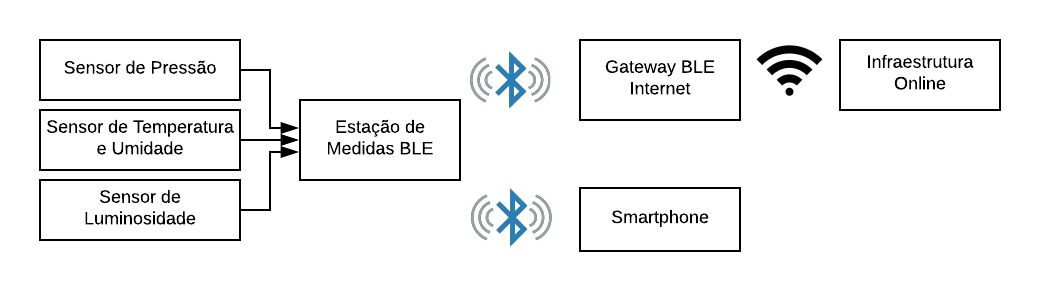
\includegraphics[width=0.5\linewidth]{project_overview.jpg}
	\captionof{figure}{Esquemático dos sistemas presentes no projeto}
	\label{fig:project_overview}
\end{center} 

O principal dispositivo bluetooth desenvolvido neste trabalho é a estação de
medidas que opera como Broadcaster e Slave, que terá suas etapas de projeto e
implementação descritas com mais detalhes.

\subsubsection{Estação de Medidas Bluetooth Low Energy}

A estação de medidas foi projetada para atender os requisitos propostos,
visando o mínimo consumo energético para possibilitar a alimentação através de
baterias sem a necessidade de manutenções frequentes.

Para a transmissão das variáveis medidas pelos sensores utiliza-se o dispositivo
no modo BLE Broadcaster, codificando os valores obtidos de forma ordenada dentro
de um pacote de advertising do bluetooth, permitindo que qualquer dispositivo
BLE próximo que seja capaz de detectar a presença da estação de medidas
receba os valores de todas as variáveis medidas.

Este método foi escolhido visando o mínimo consumo de energia por dispensar uma
conexão para a transmissão dos dados.
 
Como diferencial a estação permite a configuração de sua operação através de
serviços GATT do BLE, sendo possível alterar tanto as configurações de rádio
(potêcia e intervalo de transmissão) quanto os parâmetros de configuração dos
sensores (range, escala, intervalo entre medidas). Além disso, os serviços dos
sensores permitem o streaming das novas leituras.

\subsubsubsection{Seleção de componentes}

%TODO justificar as variáveis medidas e os critérios de seleção dos sensores,
% incluindo a disponibilidade de breakout boards

O hardware selecionado para a estação de medidas é o SoC nRF51822, produzido
pela Nordic Semiconductor. Este SoC conta com um processador ARM Cortex M0 de 32
bits e com um transceiver de 2.4GHz multiprotocolo, sendo capaz de operar com
os protocolos Bluetooth e ANT.\cite{nRF51ProdSpec}

Com o processador desligado e mantendo a memória RAM, o microcontrolador consome
uma corrente de 3.8$\mu A$,

A plataforma escolhida leva em consideração as especificações energéticas do
SoC, que é capaz de consumir uma corrente de 3.8$\mu A$ com o processador
desligado mantendo a memória RAM\cite{nRF51ProdSpec}, a possibilidade de
depuração do código desenvolvido, a versatilidade de operar tanto a aplicação
quanto o bluetooth dentro do mesmo chip e a disponibilidade do componente para o uso.

Já os sensores escolhidos para o projeto são:
\begin{itemize} 
  \item BMP180: Sensor de pressão
  \item TSL2561: Sensor de luminosidade
  \item HTU21D: Sensor de temperatura e umidade
\end{itemize}

Todos os sensores especificados são digitais e possuem características low
power. Além disso, o meio de acesso é o barramento I2C para todos os casos, fato
que auxiliou o desenvolvimento do projeto devido a interface compartilhada entre
todos os dispositivos.

\subparagraph{BMP180} O sensor BMP180, presente no placa da figura
\ref{fig:bmp180breakout} é um sensor de pressão desenvolvido, produzido e vendido pela Bosch. É capaz de
operar com tensões de 1.8V a 3.6V,consumindo uma corrente de 0.1$\mu A$ a 4$\mu
A$ nas temperaturas de $25\,^{\circ}{\rm C}$ e $85\,^{\circ}{\rm C}$ respectivamente. 
Durante a conversão dos valores de pressão, a corrente de pico varia entre
650$\mu A$ a 1000$\mu A$, e durante a operação a $25\,^{\circ}{\rm C}$ com
frequência de amostragem de 1Hz, a corrente consumida fica entre 3$\mu A$ e
32$\mu A$ dependendo da resolução do configurada.\cite{BMP180Datasheet}

\begin{center}
	\centering 
	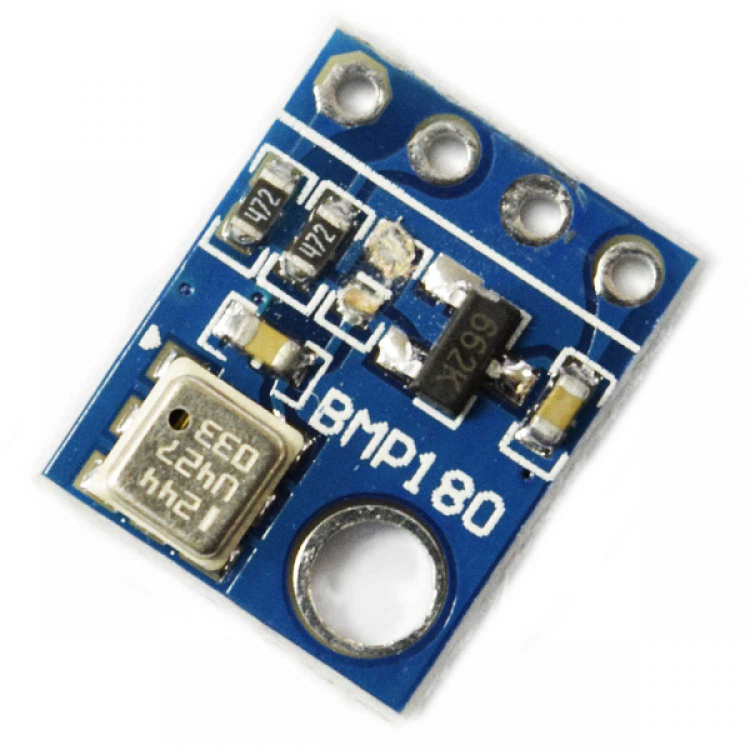
\includegraphics[width=0.5\linewidth]{BMP180.png}
	\captionof{figure}{Módulo de Desenvolvimento para o sensor BMP180}
	\label{fig:bmp180breakout}
\end{center} 


Considerando o tempo máximo de conversão para cada resolução,
estima-se que a frequência de amostragem máxima para este sensor fica entre
222.22Hz(low power mode) e 13Hz(Advanced res. mode). O range de medidas do
sensor é de 30kPa a 110kPa. \cite{BMP180Datasheet}


\subparagraph{TSL2561} O sensor TSL2561, presente na placa da figura
\ref{fig:tsl2561breakout}, é um sensor de luminosidade produzido pela empresa
ams AG que combina um fotodiodo que responde numa larga faixa espectral
(visível e infravermelho) e um fotodiodo que responde somente a faixa
infravermelha do espectro. O sensor possui comunicação I2C que permite a
configuração, leitura e envio de comandos.

\begin{center}
	\centering 
	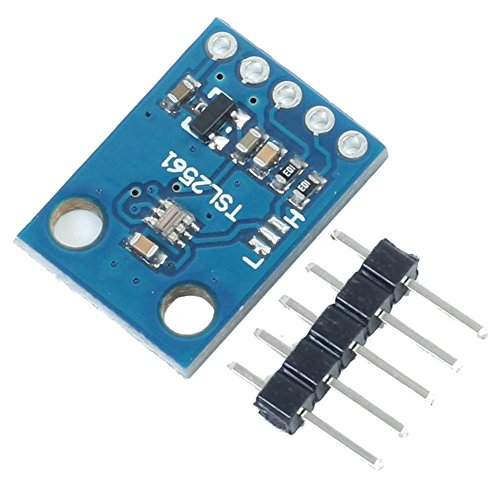
\includegraphics[width=0.4\linewidth]{TSL2561.jpg}
	\captionof{figure}{Módulo de Desenvolvimento para o sensor TSL2561}
	\label{fig:tsl2561breakout}
\end{center} 

Os valores lidos pelo sensor são convertidos para
iluminância em Lux através de uma equalção empírica fornecida pelo fabricante
que busca se aproximar da resposta do olho humano. A característica de possuir
dois fotodiodos permite com que o sensor trabalhe em regiões em que há uma
incidência alta de luz infravermelha, pois com um fotodiodo dedicado ao
infravermelho é possível medir e descontar a influência da luz infravermelha na
medida de luminosidade.\cite{TSL2561Datasheet}

A tensão de alimentação é de até 3.8V. Durante os períodos de conversão de
luminosidade, o consumo de corrente varia entre 0.24mA e 0.6mA. Já no modo
power down, o consumo de corrente varia entre 3.2$\mu A$ e 15$\mu A$. Possui
uma resolução de 16 bits na saída do ADC que realiza as conversões nos
fotodiodos. \cite{TSL2561Datasheet}


\subparagraph{HTU21D} O sensor HTU21D, presente na placa da figura
\ref{fig:htu21breakout}, é um sensor de temperatura e umidade relativa do ar
desenvolvido e produzido pela Measurement Specialities. Este sensor é low
power, sendo capaz e operar entre tensões de 1.5V e 3.6V com um consumo de
corrente variando entre 0.02$\mu A$ e 0.14$\mu A$ em standby, e consumindo uma
corrente que varia entre 300$\mu A$ a 500$\mu A$ durante a conversão de
temperatura e umidade. \cite{HTU21DDatasheet}

\begin{center}
	\centering 
	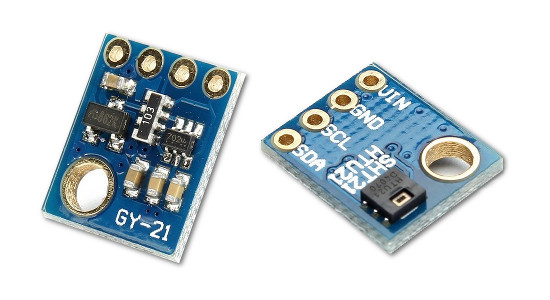
\includegraphics[width=0.4\linewidth]{HTU21.jpg}
	\captionof{figure}{Módulo de Desenvolvimento para o sensor HTU21}
	\label{fig:htu21breakout}
\end{center} 

Possui uma  resolução configurável de 8 bits a 12 bits para a medida de umidade
relativa do ar, que corresponde a 0.7\%RH e 0.04\%RH respectivamente com uma
acurácia de 2\%RH, com duração de conversão é de 3ms (8 bits) a 16ms (12 bits).
O sensor de umidade possui um tempo de resposta de 5 a 10 segundos para uma
excitação em degrau de 33\%RH para 75\%RH. \cite{HTU21DDatasheet}

Já para a medida de temperatura, a resolução é configurável entre 11 bits e 14
bits, representando $0.08\,^{\circ}{\rm C}$ e $0.01\,^{\circ}{\rm C}$
respectivamente, com uma acurácia de $0.3\,^{\circ}{\rm C}$ e com duração da
conversão variando de 7ms (11 bits) a 50ms (14 bits). Possui um tempo de
resposta de 10 segundos para uma excitação em degrau de $15\,^{\circ}{\rm C}$ a
$45\,^{\circ}{\rm C}$.\cite{HTU21DDatasheet}

\subsubsubsection{Estratégia para otimização de consumo energético}
Com a finalidade de otimizar o consumo energético foi adotada a estratégia de
manter o microcontrolador em modo deep sleep sempre que possível, sendo o mesmo
acordado somente através de interrupções para a realização das tarefas de rádio
e de leitura de sensores. Durante os períodos em sleep todos os sensores devem
estar num estado de baixo consumo de energia.\cite{MicrochipLPDesign}

Ainda na otimização do consumo, a estratégia adotada para a transmissão dos
dados dos sensores foi concepção do dispositivo operando como um BLE broadcaster
pois desta forma se reduz o período no qual há a necessidade do rádio, e
somente durante a configuração o dispositivo opera como um BLE Slave,
permitindo que uma conexão seja estabelecida e que os serviços e
características presentes sejam acessíveis.

\subsubsubsection{Parâmetros Gerais de Operação do Bluetooth}

Durante a operação, o dispositivo conterá um MAC Address do tipo Random Static
Device Address, sendo a parte aleatória do endereço definida pelo número de série do
microcontrolador. Para manter o endereço no tipo correto, é necessário garantir
que os dois bits mais significativos estejam definidos como 1. Este tipo de
endereço foi selecionado pois neste projeto não há um Identificador Único de
Organização, obtido pela IEEE Registration Authority \cite{ble4core}

\subsubsubsection{Bluetooth Broadcaster} 

Por operar no modo Broadcaster e Slave, a estação de medidas deve informar em
seus pacotes de Advertising que o dispositivo é conectável com centrais BLE,
permitindo o acesso aos serviços que serão descritos posteriormente. 

Além disso, no campo Payload do pacote transmitido através da ação de
Advertising estarão presentes as informações medidas pelos sensores, seguindo a
estrutura de dados no código fonte \ref{lst:struct_adv}. 

Como formato de payload optou-se por utilizar o Manufacturer Specific Data,
campo destinado para fabricantes desenvolverem seus próprios protocolos e
codificações, evitando assim possíveis conflitos com pacotes BLE definidos pela
especificação. Este formato possui um Data Type específico
(0xFF)\cite{GAPDataTypes}, a identificação do fabricante definida pelo
Bluetooth SIG, e os dados codificados \cite{ble4sup}. O Company ID escolhido
para o projeto é o mesmo da fabricante do microcontrolador, a Nordic
Semiconductor, que possui como registro o valor 0x0059\cite{bleCompanyIds}.

\lstinputlisting[firstline=11,lastline=18,label={lst:struct_adv},
caption={Estrutura de dados para do pacote de leituras dos sensores}]
{../Development/ble-sensor-station/src/libs/ble/advertising/ble_adv_frame.h}

No pacote de Scan Response, a estação de medidas transmitirá o seu nome,
utilizando o Data Type definido como Complete Local Name, com
código 0x09\cite{GAPDataTypes}, sendo o nome do dispositivo definido como
\dblquote{UFABC001}.

Ainda nos dados do pacote, é incluído obrigatoriamente o campo de
flags\cite{ble4core} que indicam com quais recursos do Bluetooth o dispositivo é
compatível \cite{ble4sup}, com Data Type identificado pelo byte 0x01
\cite{GAPDataTypes}.
A estação de medidas deve suportar apenas o Bluetooth Low Energy, mas não o
BR/EDR. Além disso, como o dispositivo será conectável enquanto estiver
operando, a flag General Discoverable Mode deve ser habilitada. Com estas duas
flags ativas, o campo Flags deverá conter o valor 0x06, de acordo com os bits
definidos na especificação do campo.\cite{ble4sup}.

Com todas as informações possuindo valores fixos, é possível definir a formação
do pacote de advertising, como mostra a tabela \ref{tab:adv_template}. Na
tabela, o valor final do campo Manufacturer Specific Data possui o seguinte
significado: PP para os bytes das medidas de pressão, TT para os bytes das
medidas de temperatura, HH para os bytes das medidas de umidade, VV para os
bytes das medidas de luz visível e II para os bytes referentes a luz
infravermelha. O tamanho do campo será dado pelo tamanho da estrutura de dados
somados com 3 bytes, referentes ao Company ID e ao tipo de dado. Na formação do
pacote, é importante notar que dentro do campo a ordem dos bytes e invertida,
como se observa no campo Company ID que vale 0x0059\cite{bleCompanyIds} para a Nordic
Semiconductor e no valor final passa a ser 0x5900.

\begin{table}[H]
\centering
\resizebox{\textwidth}{!}{%
\begin{tabular}{l|c|l|l|l|l|l|l|l|l|l|l|}
\cline{2-12}
                                               & \multicolumn{3}{c|}{Flags}                                                & \multicolumn{8}{c|}{Manufacturer Specific Data (MSD)}                                                         \\ \hline
\multicolumn{1}{|l|}{\multirow{2}{*}{Formato}} & \multirow{2}{*}{Tam.}     & \multirow{2}{*}{Tipo} & \multirow{2}{*}{Dado} & \multirow{2}{*}{Tam.} & \multirow{2}{*}{Tipo} & \multicolumn{6}{c|}{Dados}                                    \\ \cline{7-12} 
\multicolumn{1}{|l|}{}                         &                           &                       &                       &                       &                       & Company ID & pres    & temp    & hum     & vis\_lux & ir\_lux \\ \hline
\multicolumn{1}{|l|}{Conteúdo}                 & \multicolumn{1}{l|}{0x02} & 0x01                  & 0x06                  & 0x13                  & 0xFF                  & 0x0059     & 4 bytes & 2 bytes & 2 bytes & 4 bytes  & 4 bytes \\ \hline
\multicolumn{1}{|l|}{Valor final}              & \multicolumn{3}{c|}{0x020106}                                             & \multicolumn{8}{c|}{0x13FF5900PPPPPPPPTTTTHHHHVVVVVVVVIIIIIIII}                                               \\ \hline
\multicolumn{1}{|l|}{Pacote Final}             & \multicolumn{11}{c|}{0x02010613FF5900PPPPPPPPTTTTHHHHVVVVVVVVIIIIIIII}                                                                                                                    \\ \hline
\end{tabular}%
}
\caption{Formato do pacote de advertising}
\label{tab:adv_template}
\end{table}

O pacote enviado pelo Scan Response possui tamanho e conteúdo fixo, sendo assim
possível defini-lo, como mostra a tabela \ref{tab:scan_resp_template}.

\begin{table}[H]
\centering
\begin{tabular}{l|l|l|l|}
\cline{2-4}
                                  & \multicolumn{3}{l|}{Complete Local Name}    \\ \hline
\multicolumn{1}{|l|}{Formato}     & Tam.   & Tipo  & \multicolumn{1}{c|}{Dado}  \\ \hline
\multicolumn{1}{|l|}{Conteúdo}    & 0x09   & 0x09  & 0x5546414243303031         \\ \hline
\multicolumn{1}{|l|}{Valor final} & \multicolumn{3}{l|}{0x09095546414243303031} \\ \hline
\end{tabular}
\caption{Definição do pacote de Scan Response}
\label{tab:scan_resp_template}
\end{table}

\subsubsubsection{Bluetooth Slave}
No modo slave, o dispostivo possui um serviço Bluetooth para cada sensor, com
características que permitem a configuração dos sensores.

O UUID de 128 bits,arbitrariamente utilizado como base para
todos os serviços, está descrito no código fonte \ref{lst:base_uuid}.

\lstinputlisting[firstline=11,lastline=15,label={lst:base_uuid},
caption={Constante que define o UUID base dos serviços Bluetooth}]
{../Development/ble-sensor-station/src/libs/ble/services/ble_services_common.h}

Este UUID foi construído convertendo para hexadecimal o código ASCII da mensagem
\dblquote{UFABCIAR2018\_\_GN}, onde os caracteres \dblquote{\_\_} são os bytes
0x00 deixados em branco para o preenchimento pelo UUID específico dos serviços
bluetooth.

Foram definidos e nomeados quatro serviços Bluetooth para o dispositivo: o APSS
(Air Pressure Sensor Service), o LSS (Luminosity Sensor Service), o THSS
(Temperature and Humidity Sensor Service) e o RPCS (Radio Parameters
Configuration Service).

\newpage
\subparagraph{Air Pressure Sensor Service}(APSS) 
\newline
O APSS é o serviço responsável pela configuração e aquisição de dados do sensor
de pressão BMP180. Este sensor disponibiliza via Bluetooth as informações de
pressão atmosférica e temperatura. Este serviço possui 5 características:
Sensing Interval, Sensor Status, Sensor Resolution, Pressure Data, Temperature
Data.

Os identificadores de 2 bytes do serviço e de cada característica estão
definidos no Código Fonte \ref{lst:apss_uuid}. 

\begin{minipage}{0.95\linewidth}
\lstinputlisting[firstline=19,lastline=29,label={lst:apss_uuid},
caption={UUID para o serviço APSS e suas características}]
{../Development/ble-sensor-station/src/libs/ble/services/apss/ble_apss.h}
\end{minipage}

A característica Sensing Interval é uma característica que representa o
intervalo entre as medidas de pressão e temperatura do sensor de BMP180
configurada atualmente. Possui exatamente 4 bytes, o suficiente para armazenar
uma variável do tipo \textbf{uint32\_t}, que representa o intervalo em
milisegundos.

Ao realizar a leitura desta característica, se obtém o intervalo atual entre as
medidas do sensor, e a escrita nesta característica realiza uma nova
configuração. A leitura é permitida sem restrições, já escrita passa pelo
processo de autorização para rejeitar a configuração em caso de valor
inválido. Neste projeto não foi previsto nenhum valor inválido para o intervalo
entre as medidas, porém este recurso possibilita a implementação com menor
retrabalho de software.

A característica Sensor Status indica o estado atual do sensor. Foram previstos
3 estados diferentes para o sensor, como mostra o Código Fonte
\ref{lst:sensor_state_t}. Esta característica possui 1 byte de comprimento, que
pode ser lido a qualquer momento ou escrito com restrições. Os valores aceitos
para a escrita são 0x00 para ligar o sensor e 0x02 para
desligar o sensor.

Os valores definidos são atribuidos pela construção de uma estrutura do tipo
enumeração, sendo o primeiro elemento atribuido com o valor inteiro 0, e
cada novo elemento soma-se 1 unidade ao valor atribuído, conforme
a especificação do enum para a linguagem C.\cite{C99Spec}

\begin{minipage}{0.95\linewidth}
\lstinputlisting[firstline=42,lastline=47,label={lst:sensor_state_t},
caption={Enumeração dos possíveis estados para o sensor}]
{../Development/ble-sensor-station/src/libs/sensing/sensor_public_interface.h}
\end{minipage}

A característica Sensor Resolution determina a resolução e o modo de operação do
sensor. Nesta característica com comprimento de 1 byte, permite-se a leitura sem
restrições e a escrita com validação do valor configurado. Os valores aceitos
para a escrita estão definidos pela enumeração do Código Fonte \ref{lst:bmp180_pwr_mode_t}.
\cite{BMP180Datasheet}

\begin{minipage}{0.95\linewidth}
\lstinputlisting[firstline=14,lastline=21,label={lst:bmp180_pwr_mode_t},
caption={Enumeração dos modos de operação configuráveis para o sensor BMP180}]
{../Development/ble-sensor-station/src/libs/sensing/bmp180_drv/bmp180_drv.h}
\end{minipage}

As características Pressure Data e Temperature Data são responsáveis pela
transmissão das leituras realizadas pelos sensores. Nelas, armazena-se somente a
leitura mais recente dos sensores sem o acesso ao histórico de leituras. Estas
características permitem apenas a leitura, sem a possibilidade de escrita.
Também está habilitado o recurso de Notify, que permite a transmissão dos
dados lidos dos sensores para o dispositivo conectado sem uma solicação de
leitura, operando num sistema de streaming de dados sempre que uma nova leitura
é realizada.

A característica Pressure Data possui 4 bytes de comprimento, transmitindo os
dados num formato \textbf{uint32\_t}, representando a pressão atmosférica em Pa.
Já a Temperature Data, o comprimento é de 2 bytes, transmitindo a temperatura
num formato \textbf{int16\_t}, sendo que cada unidade representa
$0.01\,^{\circ}{\rm C}$ 

A figura \ref{fig:resumo_apss} representa graficamente a construção do serviço
Air Pressure Sensor Service.

\begin{tcolorbox}[arc=3mm,fontupper=\small,fonttitle=\bfseries,
subtitle style={boxrule=0.4pt, colback=white},colframe=green!25!black,
halign=center,bottom=0mm,
title=Air Pressure Sensor Service]
	\setstretch{1.0}
	UUID de 2 bytes do serviço: 0xABC1h
	
	\begin{tcbitemize}[raster columns=2,raster equal height,fontupper=\footnotesize,
	colbacktitle=yellow!100!red!100!black, coltitle=black,
	fonttitle=\footnotesize\bfseries,size=small, halign=center]
	
	\tcbitem [squeezed title={Sensing Interval Characteristic}]
		\begin{tabular}{ r | l }
		UUID & 0x0A00h \\ \hline
		Tamanho & 4 bytes \\ \hline
		Leitura & Permitida \\ \hline
		Escrita & Permitida com autorização \\ \hline
		Notificação & Desabilitada 
		\end{tabular}

		\tcbitem [squeezed title={Sensor Status Characteristic}]
		\begin{tabular}{ r | l }
		UUID & 0x0A01h \\ \hline
		Tamanho & 1 byte \\ \hline
		Leitura & Permitida \\ \hline
		Escrita & Permitida com autorização \\ \hline
		Notificação & Desabilitada 
		\end{tabular}
		
		\tcbitem [squeezed title={Sensor Resolution Characteristic}]
		\begin{tabular}{ r | l }
		UUID & 0x0A02h \\ \hline
		Tamanho & 1 byte \\ \hline
		Leitura & Permitida \\ \hline
		Escrita & Permitida com autorização \\ \hline
		Notificação & Desabilitada 
		\end{tabular}

		\tcbitem [squeezed title={Pressure Data Characteristic}]
		\begin{tabular}{ r | l }
		UUID & 0x0A03h \\ \hline
		Tamanho & 4 bytes \\ \hline
		Leitura & Permitida \\ \hline
		Escrita & Não permitida \\ \hline
		Notificação & Habilitada 
		\end{tabular}
		
		\tcbitem [squeezed title={Temperature Data Characteristic}]
		\begin{tabular}{ r | l }
		UUID & 0x0A04h \\ \hline
		Tamanho & 2 bytes \\ \hline
		Leitura & Permitida \\ \hline
		Escrita & Não permitida \\ \hline
		Notificação & Habilitada 
		\end{tabular}		
	\end{tcbitemize}
	\tcblower
	\captionof{figure}{Resumo da definição do serviço APSS}\label{fig:resumo_apss}
\end{tcolorbox}

\newpage
\subparagraph{Temperature and Humidity Sensor Service}(THSS) 
\newline

O THSS é o serviço de configuração e aquisição de dados do sensor HTU21D, que
disponibiliza as leituras de temperatura e umidade relativa do ar. O serviço
possui 5 características: Sensing Interval, Sensor Status, Sensor Resolution,
Temperature Data e Humidity Data.

O indentificador de 2 bytes do serviço e de cada característica estão
disponíveis no código fonte \ref{lst:thss_uuid}.

\begin{minipage}{0.95\linewidth}
\lstinputlisting[firstline=22,lastline=28,label={lst:thss_uuid},
caption={UUID para o serviço THSS e suas características}]
{../Development/ble-sensor-station/src/libs/ble/services/thss/ble_thss.h}
\end{minipage}

As características Sensing Interval e Sensor Status seguem as mesmas
especificações do serviço APSS.

A característica Sensor Resolution é uma característica de 1 byte permite a
configuração e leitura da resolução das medidas de temperatura e umidade. As
resoluções das medidas são dependentes uma da outra, sendo as combinações
definidas pelo fabricante. O código fonte \ref{lst:htu21d_resolution_t} reflete
as opções de resolução oferecidas. Os números indicados na resolução
representam o número de bits.

\begin{minipage}{0.95\linewidth}
\lstinputlisting[firstline=14,lastline=20,label={lst:htu21d_resolution_t},
caption={Enumeração das combinações de resolução do HTU21D}]
{../Development/ble-sensor-station/src/libs/sensing/htu21d_drv/htu21d_drv.h}
\end{minipage}

As características Temperature Data e Humidity Data seguem os mesmos padrões de
apresentação de dados do serviço APSS, sendo possível somente a leitura com
possibilidade de notificação. Ambas possuem o tamanho de 2 bytes, sendo que a
temperatura é transmitida no formato \textbf{int16\_t} enquanto a umidade segue
o formato \textbf{uint16\_t}.

Para a temperatura a unidade transmitida é centésimos de $^{\circ}{\rm C}$,
enquanto a umidade relativa é transmitida em centésimos de \%RH. A conversão de
unidades foi feita para possibilitar a transmissão dos valores com as precisões
lidas pelos sensores sem a necessidade de utilizar ponto flutuante no software e
sem prejuízo aos dados.

A figura \ref{fig:resumo_thss} representa graficamente a construção do serviço
Temperature and Humidity Sensor Service

\begin{tcolorbox}[arc=3mm,fontupper=\small,fonttitle=\bfseries,
subtitle style={boxrule=0.4pt, colback=white},colframe=green!25!black,
halign=center,bottom=0mm,
title=Temperature and Humidity Sensor Service]
	\setstretch{1.0}
	UUID de 2 bytes do serviço: 0xABC2h
	
	\begin{tcbitemize}[raster columns=2,raster equal height,fontupper=\footnotesize,
	colbacktitle=yellow!100!red!100!black, coltitle=black,
	fonttitle=\footnotesize\bfseries,size=small, halign=center]
	
	\tcbitem [squeezed title={Sensing Interval Characteristic}]
		\begin{tabular}{ r | l }
		UUID & 0x0B00h \\ \hline
		Tamanho & 4 bytes \\ \hline
		Leitura & Permitida \\ \hline
		Escrita & Permitida com autorização \\ \hline
		Notificação & Desabilitada 
		\end{tabular}

		\tcbitem [squeezed title={Sensor Status Characteristic}]
		\begin{tabular}{ r | l }
		UUID & 0x0B01h \\ \hline
		Tamanho & 1 byte \\ \hline
		Leitura & Permitida \\ \hline
		Escrita & Permitida com autorização \\ \hline
		Notificação & Desabilitada 
		\end{tabular}
		
		\tcbitem [squeezed title={Sensor Resolution Characteristic}]
		\begin{tabular}{ r | l }
		UUID & 0x0B02h \\ \hline
		Tamanho & 1 byte \\ \hline
		Leitura & Permitida \\ \hline
		Escrita & Permitida com autorização \\ \hline
		Notificação & Desabilitada 
		\end{tabular}

		\tcbitem [squeezed title={Temperature Data Characteristic}]
		\begin{tabular}{ r | l }
		UUID & 0x0B03h \\ \hline
		Tamanho & 2 bytes \\ \hline
		Leitura & Permitida \\ \hline
		Escrita & Não permitida \\ \hline
		Notificação & Habilitada 
		\end{tabular}
		
		\tcbitem [squeezed title={Humidity Data Characteristic}]
		\begin{tabular}{ r | l }
		UUID & 0x0B04h \\ \hline
		Tamanho & 2 bytes \\ \hline
		Leitura & Permitida \\ \hline
		Escrita & Não permitida \\ \hline
		Notificação & Habilitada 
		\end{tabular}		
	\end{tcbitemize}
	\tcblower
	\captionof{figure}{Resumo da definição do serviço THSS}\label{fig:resumo_thss}
\end{tcolorbox}

\newpage
\subparagraph{Luminosity Sensor Service}(LSS) 
\newline
O LSS é o serviço de configuração e aquisição de dados do sensor TSL2561. O
sensor disponibiliza as leituras de luminosidade no espectro visível e
luminosidade no espectro infravermelho. Este serviço possui 6 características:
Sensing Interval; Sensor Status; Integration Time; Sensor Gain; Visible Lux
Data e  Infrared Lux Data.

Os identificadores de 2 bytes do serviço e de cada característica estão
definidos no Código Fonte \ref{lst:lss_uuid}. 

\begin{minipage}{0.95\linewidth}
\lstinputlisting[firstline=22,lastline=29,label={lst:lss_uuid},
caption={UUID para o serviço LSS e suas características}]
{../Development/ble-sensor-station/src/libs/ble/services/lss/ble_lss.h}
\end{minipage}

As características Sensing Interval e Sensor Status seguem as mesmas
especificações do serviço APSS.

A característica Integration Time configura a janela de amostragem do sensor.
Esta característica permite a leitura do valor atual e permite a escrita com
restrição, já que o sensor possui configurações pré definidas (13.7 ms, 101 ms
ou 402 ms). O Código Fonte \ref{lst:tsl2561_integration_time_t} define os
valores aceitos para escrita nesta característica. \cite{TSL2561Datasheet}

\begin{minipage}{0.95\linewidth}
\lstinputlisting[firstline=14,lastline=19,label={lst:tsl2561_integration_time_t},
caption={Enumeração dos tempos de integração disponíveis para o TSL2561}]
{../Development/ble-sensor-station/src/libs/sensing/tsl2561_drv/tsl2561_drv.h}
\end{minipage}

A característica Sensor Gain permite a configuração e leitura do valor atual do
ganho interno do sensor, que pode ser 0 (sem ganho) ou 16 vezes. A escrita é
permitida com restrição por permitir apenas dois valores. O Código Fonte
\ref{lst:tsl2561_gain_t} define os valores aceitos para escrita nesta
característica.

\begin{minipage}{0.95\linewidth} 
\lstinputlisting[firstline=21,lastline=25,label={lst:tsl2561_gain_t},
caption={Enumeração das opções de ganho para o TSL2561}]
{../Development/ble-sensor-station/src/libs/sensing/tsl2561_drv/tsl2561_drv.h}
\end{minipage}

As características Visible Lux Data e Infrared Lux Data seguem o mesmo padrão
dos outros serviços para a apresentação dos dados, mantendo a última leitura e
com o recurso de Notify habilitado.

Ambas as características possuem 4 bytes de comprimento, transmitindo os dados
num formato \textbf{uint32\_t}, representando as luminosidades correspondentes
em Lux.

A figura \ref{fig:resumo_lss} representa graficamente a construção do serviço
Luminosity Sensor Service.

\begin{tcolorbox}[arc=3mm,fontupper=\small,fonttitle=\bfseries,
subtitle style={boxrule=0.4pt, colback=white},colframe=green!25!black,
halign=center,bottom=0mm,
title=Luminosity Sensor Service]
	\setstretch{1.0}
	UUID de 2 bytes do serviço: 0xABC3h
	
	\begin{tcbitemize}[raster columns=2,raster equal height,fontupper=\footnotesize,
	colbacktitle=yellow!100!red!100!black, coltitle=black,
	fonttitle=\footnotesize\bfseries,size=small, halign=center]
	
	\tcbitem [squeezed title={Sensing Interval Characteristic}]
		\begin{tabular}{ r | l }
		UUID & 0x0C00h \\ \hline
		Tamanho & 4 bytes \\ \hline
		Leitura & Permitida \\ \hline
		Escrita & Permitida com autorização \\ \hline
		Notificação & Desabilitada 
		\end{tabular}

		\tcbitem [squeezed title={Sensor Status Characteristic}]
		\begin{tabular}{ r | l }
		UUID & 0x0C01h \\ \hline
		Tamanho & 1 byte \\ \hline
		Leitura & Permitida \\ \hline
		Escrita & Permitida com autorização \\ \hline
		Notificação & Desabilitada 
		\end{tabular}
		
		\tcbitem [squeezed title={Sensor Integration Time Characteristic}]
		\begin{tabular}{ r | l }
		UUID & 0x0C02h \\ \hline
		Tamanho & 1 byte \\ \hline
		Leitura & Permitida \\ \hline
		Escrita & Permitida com autorização \\ \hline
		Notificação & Desabilitada 
		\end{tabular}
		
		\tcbitem [squeezed title={Sensor Gain Characteristic}]
		\begin{tabular}{ r | l }
		UUID & 0x0C03h \\ \hline
		Tamanho & 1 byte \\ \hline
		Leitura & Permitida \\ \hline
		Escrita & Permitida com autorização \\ \hline
		Notificação & Desabilitada 
		\end{tabular}

		\tcbitem [squeezed title={Pressure Data Characteristic}]
		\begin{tabular}{ r | l }
		UUID & 0x0C04h \\ \hline
		Tamanho & 4 bytes \\ \hline
		Leitura & Permitida \\ \hline
		Escrita & Não permitida \\ \hline
		Notificação & Habilitada 
		\end{tabular}
		
		\tcbitem [squeezed title={Temperature Data Characteristic}]
		\begin{tabular}{ r | l }
		UUID & 0x0C05h \\ \hline
		Tamanho & 4 bytes \\ \hline
		Leitura & Permitida \\ \hline
		Escrita & Não permitida \\ \hline
		Notificação & Habilitada 
		\end{tabular}		
	\end{tcbitemize}
	\tcblower
	\captionof{figure}{Resumo da definição do serviço LSS}\label{fig:resumo_lss}
\end{tcolorbox}

\newpage
\subparagraph{Radio Parameters Configuration Service}(RPCS) 
\newline
O RPCS é o serviço de configuração dos parâmetros de operação do rádio,
oferecendo a possibilidade de configurar o intervalo de transmissão de
advertisings e a potência de transmissão do rádio. Este serviço possui 2
características: Advertising Interval e Advertising TX Power.

Os identificadores de 2 bytes do serviço e de cada característica estão
definidos no Código Fonte \ref{lst:rpcs_uuid}. 

\begin{minipage}{0.95\linewidth}
\lstinputlisting[firstline=11,lastline=14,label={lst:rpcs_uuid},
caption={UUID para o serviço RPCS e suas características}]
{../Development/ble-sensor-station/src/libs/ble/services/rpcs/ble_rpcs.h}
\end{minipage}

Devido às especificações impostas pelo Bluetooh, o intervalo de advertising só
pode ser configurado entre 20ms e 10240ms\cite{ble4core}. A característica que
configura este parâmetro possui um tamanho de 2 bytes permite a leitura e
escrita com autorização, que somente autoriza a escrita de valores válidos. Os
valores escritos representam o intervalo em milisegundos, representados por uma
variável do tipo \textbf{uint16\_t}.

Já a configuração da potência do rádio só é capaz de receber as configurações
permitidas pelo microcontrolador, que são: +4dB, 0dB, -4dB, -8dB, -12dB, -16dB e
-20dB\cite{nRF51RefManual}. A característica que configura este parâmetro possui
1 byte, seguindo o formato \textbf{int8\_t}, e permite a leitura e escrita com
autorização, permitindo apenas a escrita de valores válidos. O valor escrito
representa a potência de transmissão em decibels.

A figura \ref{fig:resumo_rpcs} representa graficamente a construção do serviço
Radio Parameters Configuration Service.

\begin{tcolorbox}[arc=3mm,fontupper=\small,fonttitle=\bfseries,
subtitle style={boxrule=0.4pt, colback=white},colframe=green!25!black,
halign=center,bottom=0mm,
title=Radio Parameter Configuration Service]
	\setstretch{1.0}
	UUID de 2 bytes do serviço: 0xABC4h
	
	\begin{tcbitemize}[raster columns=2,raster equal height,fontupper=\footnotesize,
	colbacktitle=yellow!100!red!100!black, coltitle=black,
	fonttitle=\footnotesize\bfseries,size=small, halign=center]
	
	\tcbitem [squeezed title={Advertising Interval Characteristic}]
		\begin{tabular}{ r | l }
		UUID & 0x0D00h \\ \hline
		Tamanho & 4 bytes \\ \hline
		Leitura & Permitida \\ \hline
		Escrita & Permitida com autorização \\ \hline
		Notificação & Desabilitada 
		\end{tabular}

		\tcbitem [squeezed title={Advertising TX Power Characteristic}]
		\begin{tabular}{ r | l }
		UUID & 0x0D01h \\ \hline
		Tamanho & 1 byte \\ \hline
		Leitura & Permitida \\ \hline
		Escrita & Permitida com autorização \\ \hline
		Notificação & Desabilitada 
		\end{tabular}

	\end{tcbitemize}
	\tcblower
	\captionof{figure}{Resumo da definição do serviço RPCS}
	\label{fig:resumo_rpcs}
\end{tcolorbox}

%End of Sensor Station

\subsubsection{Infraestrutura online}

A infraestrutura online escolhida foi o AWS IoT Core, oferecido pela Amazon Web
Services. O AWS IoT Core é uma plataforma que permite a conexão de dispositivos
a aplicativos de nuvem que possui alta capacidade de tráfego de dados, sendo
capaz também de processar e rotear os dados para outros serviços online.
\cite{AWS_IoTCore}

\subsubsubsection{Serviço para recepção de mensagens}

O AWS IoT Core oferece um dashboard online que permite a criação de dispositivos.

%end of infrastructure

\subsubsection{Gateway Bluetooth - Internet}

\subsubsubsection{Especificação}

O Gateway Bluetooth - Internet é o dispositivo responsável por monitorar os
pacotes BLE presentes no ar, indentificar o pacote específico transmitido pela
estação de medidas, decodificá-lo e enviá-lo para a infraestrutura online.

Este dispositivo deverá se manter conectado a internet, seja por rede cabeada
ou através de Wi-Fi, e ao mesmo tempo se manter como um BLE Observer, captando os
pacotes bluetooth.

Ao decodificar os pacotes alvo, o envio para a internet se dará pelo protocolo MQTT,
que é oferecido como interface na infraestrutura online.

\subsubsubsection{Hardware escolhido}

%TODO SoC
O hardware escolhido foi SoC ESP32, produzido pela Espressif Systems, que já possui
comunicação via Wi-Fi e BLE integrado ao chip, sendo possível utilizar as duas funções
simultaneamente. A placa de desenvolvimento utilizada é a ESP32-DevKitC,
mostrada na figura \ref{fig:nodemcu32}.\cite{ESP32Datasheet}

\begin{center}
	\centering 
	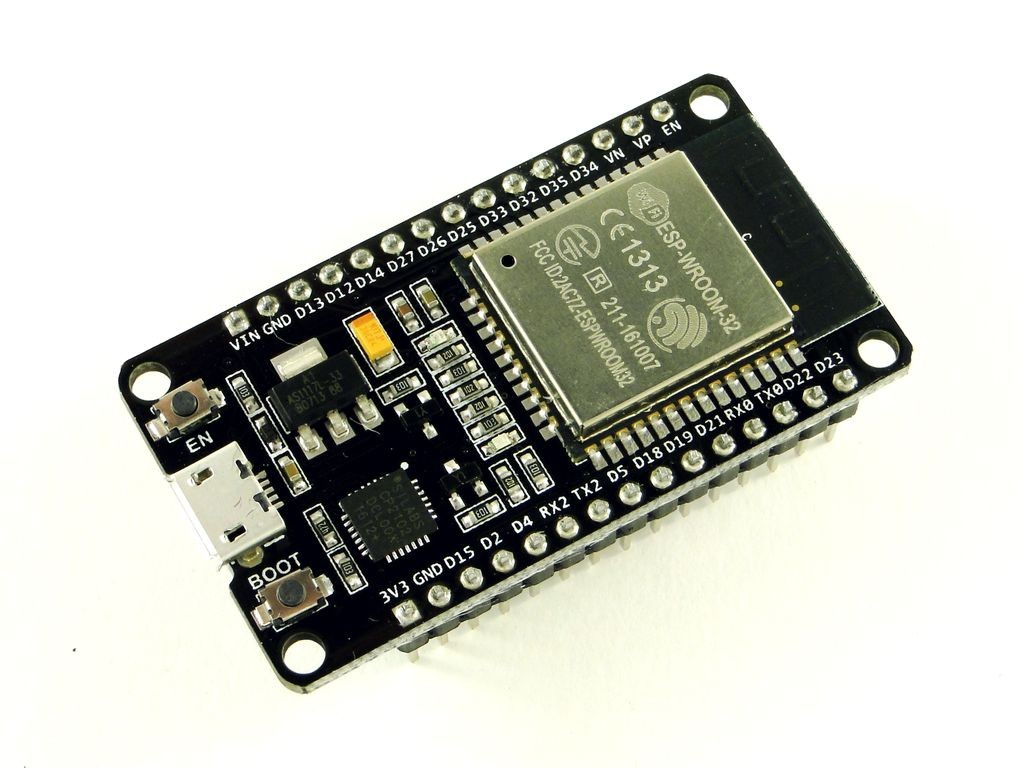
\includegraphics[width=0.8\linewidth]{nodemcu32.jpg}
	\captionof{figure}{Placa de desenvolvimento ESP32-DevKitC}
	\label{fig:nodemcu32}
\end{center} 

%TODO SDK, FREE RTOS
O SDK do fabricante, chamado de ESP-IDF (Espressif IoT Development Framework),
oferece exemplos de utilização do Bluetooth, Wi-Fi, e também disponibiliza de
forma gratuita o sistema operacional para sistemas embarcados Amazon FREE-RTOS,
uma versão do FREE-RTOS customizada pela Amazon, que amplia as funcionalidades
com bibliotecas de software que auxiliam a conexão de sistemas embarcados com
os serviços de nuvem AWS.

Além destas facilidades, este SoC foi selecionado pela sua disponibilidade no
mercado a preços acessíveis e por tratar-se de um componente relativamente
novo no mercado, sendo lançado somente em 2016\cite{ESP32Datasheet}. 

Com a utilização do kit de desenvolvimento não há a necessidade de ligar nenhum
outro componente ao ESP32.

\subsubsubsection{Bluetooth Observer}

O em relação ao Bluetooth, Gateway Bluetooth - Internet deverá operar o tempo
todo como um Bluetooth Observer. A amostragem será em tempo integral, sem a
utilização de janelamento.

Ao detectar um pacote de Advertising é papel deste dispositivo detectar se a
origem desse pacote é da Estação de Medidas desenvolvida neste trabalho, e esta
detecção será feita através da identificação do pacote como Manufacturer
Specific Data com o Company ID da Nordic Semiconductor. 

Após identificado, o pacote deverá ser decodificado e organizado numa estrutura
de dados que será disponibilizada para as funcionalidades de internet do
dispositivo.

\subsubsubsection{Conectividade}

Na parte de conectividade com a internet, o Gateway Bluetooth - Internet deve
ser capaz de se conectar a uma rede Wi-Fi de 2.4GHz pré definida na compilação
do código.

Após a conexão, o dispositivo irá se conectar e autenticar de forma segura aos
serviços da Amazon AWS, utilizando para isso uma chave privada e um certificado
digital, ambos na armazenados memória não volátil do microcontrolador durante a
gravação do programa. A chave privada e o certificado digital são utilizados
para a comunicação criptografada entre o microcontrolador e os serviços
online \cite{AWS_IoTCore}.

%TODO mqtt
Após conectado, o dispositivo enviará os dados dos sensores que foram obtidos
através dos pacotes de advertising para o serviço Amazon AWS IoT Core através do
protocolo MQTT.

\subsection{Implementação}

\subsubsection{Estação de Medidas Bluetooth Low Energy}

\subsubsubsection{Hardware}

Na montagem física deste projeto foi utilizado o kit de desenvolvimento
comercializado online sob o nome BLE400, que é um kit de desenvolvimento para o
microcontrolador deste projeto e oferece uma placa de circuito impresso
montada com o microcontrolador e o circuito de rádio. Junto a essa placa, há uma
segunda placa com um soquete para a placa com o circuito de rádio que oferece
diversas conexões (SPI, I2C e UART), LEDs, botões, uma interface USB-Serial e
uma interface para a gravação do microcontrolador. A figura \ref{fig:BLE400}
mostra a foto do kit de desenvolvimento.

\begin{center}
	\centering 
	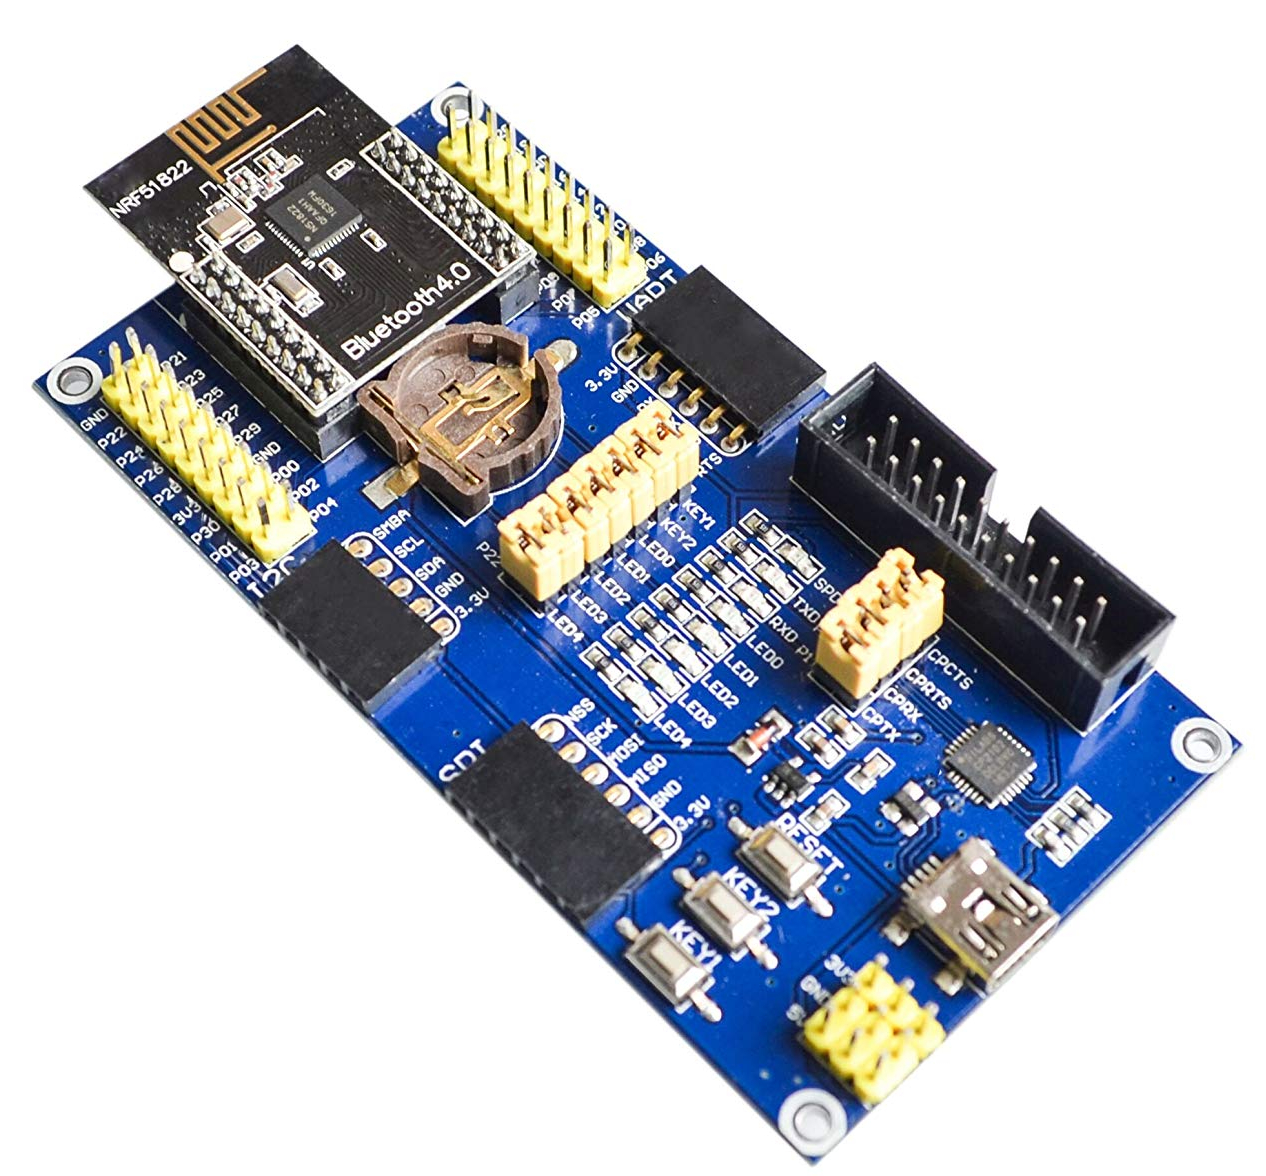
\includegraphics[width=0.6\linewidth]{BLE400.jpg}  
	\captionof{figure}{Kit de Desenvolvimento BLE400}
	\label{fig:BLE400}
\end{center} 

Junto a esse kit, foi montada uma outra placa de circuito, desta vez em placa
padrão, que oferece uma conexão para as placas de desenvolvimento dos sensores
mostradas na seção \ref{subsection:projeto}, como mostra a figura
\ref{fig:custom_board}. Esta placa oferece um barramento I2C que se conecta ao
barramento I2C oferecido pelo kit de desenvolvimento do microcontrolador.

\begin{center}
	\centering 
	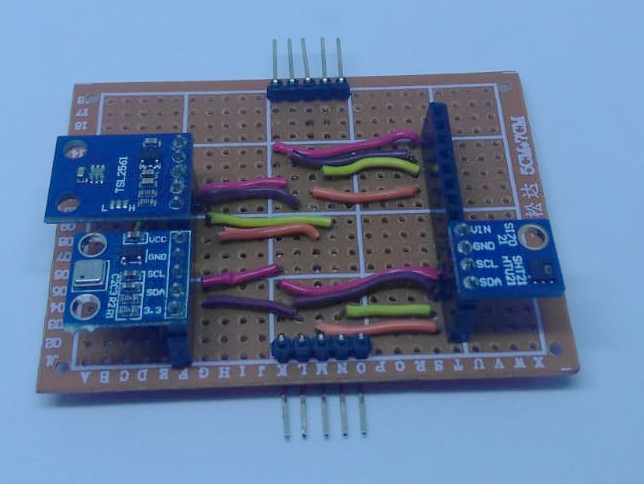
\includegraphics[width=0.8\linewidth]{custom_pcb.jpeg}
	\captionof{figure}{Placa padrão montada para o projeto}
	\label{fig:custom_board}
\end{center} 

A figura \ref{fig:mounted_proj} mostra uma foto das duas placas conectadas.

\begin{center}
	\centering 
	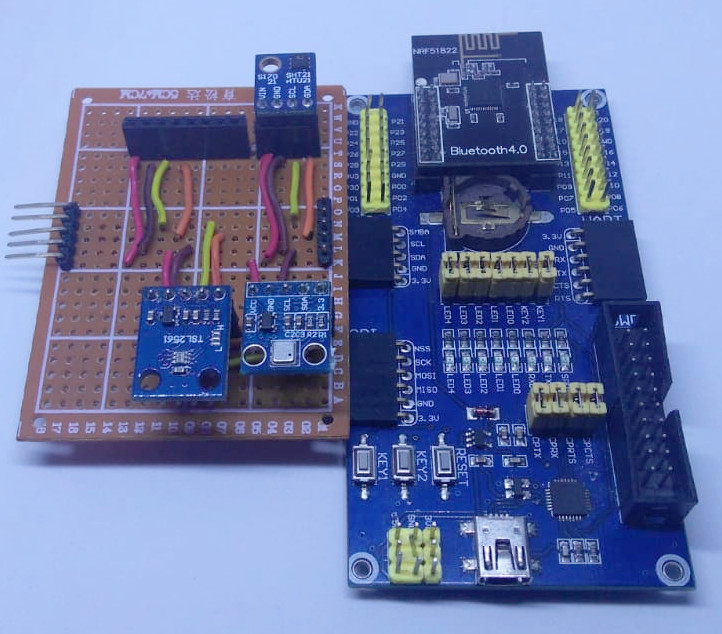
\includegraphics[width=0.9\linewidth]{mounted.jpeg} 
	\captionof{figure}{Placas do projeto montadas}
	\label{fig:mounted_proj}
\end{center} 


\subsubsubsection{Ambiente de desenvolvimento}

O ambiente de desenvolvimento foi baseado no Software Development Kit oferecido
pelo fabricante do microcontrolador, o nRF5 SDK 12.3. Este SDK acelera o
desenvolvimento do projeto por diminuir a necessidade de acesso direto aos
registradores do microcontrolador para a operação de hardware, permitindo uma
programação em nível mais alto.
 
O projeto de firmware foi feito utilizando-se Makefile e o toolchain ARM-GCC,
permitindo assim o desenvolvimento e compilação do projeto de forma
independente de IDE e de forma totalmente gratuita sem limitações quanto ao
tamanho do arquivo gerado ou número de linhas e arquivos de projeto.
Há também a possibilidade de desenvolvimento com a
IDE Keil, que é especifica para microcontroladores ARM.

A IDE utilizada ao para o desenvolvimento foi o Eclipse IDE versão Oxygen. Além
disso, foram necessárias as ferramentas NRFJPROG, software desenvolvido pelo
fabricante do microcontrolador para realizar tarefas como gravação, leitura,
apagar memória, etc., e a ferramenta Segger J-Link, como interface entre o
computador e o microcontrolador para as operações do NRFJPROG e para a
depuração do firmware. A Nordic Semiconductor oferece em seu site de suporte para desenvolvedores 
instruções para replicar este ambiente de desenvolvimento
\cite{devzoneGccEclipse}. Para a gravação, há também a opção de se utilizar o
software nFR GO Studio, também desenvolvido e distribuido pela Nordic
Semiconductor.

A vantagem da utilização das ferramentas NRFJPROG em conjunto com o J-Link e o
Eclipse é a possibilidade de depuração do código.

O makefile é o arquivo destinado a automação da compilação de todos os
componentes de software envolvidos no projeto. Nele foram definidos todos os
arquivos que são compilados no projeto, como mostra o código fonte
\ref{lst:make_proj_files}, bem como todas as instruções dadas ao compilador no
formato de flags de compilação, como mostra o código fonte \ref{lst:make_flags}

\begin{minipage}{0.95\linewidth} 
\lstinputlisting[firstline=11,lastline=25,label={lst:make_proj_files},
caption={Lista dos arquivos de projeto para compilação}] 
{../Development/ble-sensor-station/Makefile}
\end{minipage}

\begin{minipage}{0.95\linewidth} 
\lstinputlisting[firstline=115,lastline=133,label={lst:make_flags},
caption={Flags de compilação comuns a todos os arquivos}] 
{../Development/ble-sensor-station/Makefile}
\end{minipage}
 
%TODO definir SDK
Os arquivos com o caminho iniciado com \dblquote{\$(PROJ\_DIR)} são referentes
aos arquivos de projeto produzidos ao longo deste trabalho, enquanto os arquivos
com caminho iniciado com \dblquote{\$(SDK\_DIR)} são arquivos do Software
Development Kit oferecido pelo fabricante, e \dblquote{\$(PROJ\_DIR)} e
\dblquote{\$(SDK\_DIR)} são variáveis definidas no início do arquivo indicando a
localização da pasta de projeto e da pasta do SDK.

Para a inicialização do projeto é disponibilizado no próprio SDK, na pasta de
exemplos, um template de projeto que contém o Makefile adequado bem como o
arquivo \dblquote{main.c}, sendo o primeiro passo customizar as bibliotecas
utilizadas que devem ser compiladas, bem como as informações de projeto
presentes no Makefile, como ajustes de nomes de pastas e de flags de compilação
quando aplicável. Este Makefile já vem com algumas opções prontas. São elas:

\begin{itemize}
  \item \textbf{make default} ou \textbf{make}: compila o programa
  \item \textbf{make flash}: compila e grava o programa no microcontrolador
  \item \textbf{make clean}: apaga todos os objetos compilados
\end{itemize}

Para executar as funções do Makefile, basta navegar até a pasta onde o arquivo
está e executar os comandos oferecidos.

Em computadores com sistema operacional Windows, é necessária a instalação de
algum software Make, como o \dblquote{GNU Make for Windows}, bem como a adição
do programa às variáveis de ambiente do sistema.

É importante ressaltar que este SDK não oferece as bibliotecas de
baixo nível para a operação do rádio e do bluetooth. Para a utilização do bluetooth, o
fabricante oferece um arquivo pré compilado chamado SoftDevice, que deve ser
gravado no microcontrolador junto com o programa da aplicação. O Makefile
oferecido no template de projeto já prevê um comando para gravar o softdevice,
através do comando \dblquote{\textbf{make flash\_softdevice}}. Neste projeto,
utilizou-se o SoftDevice S130.

% TODO focar no como
% explicar o passo a passo melhor

\subsubsubsection{Arquitetura de Software}

A etapa de elaboração de arquitetura foi desempenhada para permitir melhor
organização, planejamento, atribuição de responsabilidades e testes das
funcionalidades.
Assim é possível ter uma visão do todo antes da implementação do software do dispositivo.

A arquitetura de software segue o esquema presente na figura
\ref{fig:architecture}.

\begin{center}
	\centering 
	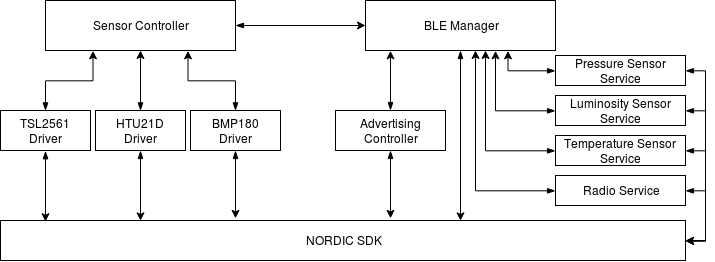
\includegraphics[width=0.9\linewidth]{Arquitetura.png}
	\captionof{figure}{Arquitetura com todos os módulos do Software}
	\label{fig:architecture}
\end{center} 

Com exceção do componente \dblquote{NORDIC SDK}, todos os componentes de
software foram implementados neste projeto, sendo cada um responsável por alguma
tarefa específica.

Os drivers para sensores são os componentes de software responsáveis por
interagir com cada um dos sensores. Neles, estão as funcionalidades de enviar
comandos ao sensor, realizar a leitura das informações do sensor e realizar os
cálculos necessários para se obter o valor das variáveis medidas.

Os quatro serviços indicados são os serviços descritos na seção
\ref{subsection:projeto}. A implementação dos serviços é responsável tanto pela
alocação das características dos serviços quanto pelo comportamento do
dispositivo durante a conexão, escrita e leitura de serviços e streaming de
dados para as notificações.

%TODO sigla MSD
O Advertising Controller é o elemento responsável construção do pacote de
advertising, codificando do dados dos sensores no pacote, preenchendo os
metadados do pacote como indicar a formatação MSD dos dados, indicação de
advertising público e indicação de dispositivo conectável, bem como preencher os
dados que serão transmitidos na solicitação do pacote Scan Response.

O Sensor Controller é o elemento responsável por gerenciar todos os sensores por
meio dos drivers disponíveis. As responsabilidades dele são solicitar as
leituras de sensores periódicamente sendo que cada sensor possui uma
configuração específica, configurar o sensor quando seu respectivo serviço
bluetooth soliciar, processar os eventos de dados prontos dos sensores e
disponibilizar para os outros módulos as medidas mais recentes feitas
pelos sensores.

%TODO sigla BLE, MAC
O BLE Manager é o elemento responsável pela configuração dos elementos básicos
de rádio, como endereço MAC, parâmetros de conexão, inicialização do protocolo e
das funcionalidades de rádio, de instanciar os serviços e de distribuir os
eventos de sensores e eventos do Bluetooth para os serviços e o Advertising
Controller.

\subsubsubsection{Operação dos sensores}

Toda operação de aquisição de dados ou de configuração realizada pelos sensores
é controlada pelo módulo Sensor Controller, que oferece uma interface para a
configurar, ligar ou desligar e definir o período de amostragem dos sensores. O
código fonte \ref{lst:sensor_controller_interface} mostra a interface oferecida
no arquivo \dblquote{sensor\_controller.h}.
 
\begin{minipage}{0.95\linewidth} 
\lstinputlisting[firstline=107,lastline=141,label={lst:sensor_controller_interface},
caption={Interface criada para acesso aos
sensores},basicstyle=\scriptsize\ttfamily]
{../Development/ble-sensor-station/src/libs/sensing/sensor_controller.h}
\end{minipage}

Na inicialização, todos os sensores são configurados com os valores padrão que
são definidos no momento da compilação e seus respectivos timers inicializam. O
código fonte \ref{lst:pressure_init} mostra o código de inicialização para o
sensor de pressão presente no arquivo \dblquote{sensor\_controller.c}. O mesmo
padrão é seguido para os outros sensores.

\begin{minipage}{0.95\linewidth} 
\lstinputlisting[firstline=66,lastline=87,label={lst:pressure_init},
caption={Inicialização do sensor de pressão}] 
{../Development/ble-sensor-station/src/libs/sensing/sensor_controller.c}
\end{minipage}

Para manter a orientação a eventos, os sensores são acessados para
leitura somente quando há um evento de estouro do timer relacionado àquele
sensor, eliminando a utilização de delays dentro do programa. 

Na ocorrência deste evento, o Sensor Controller envia um comando de
leitura para o driver do sensor, que por sua vez aciona o sensor e
preparar um timer que estoura somente quando o sensor concluir o processo
de medição, mantendo assim o microcontrolador em modo sleep enquanto o sensor
opera. Este esquema de operação é mostrado no diagrama de sequência da figura
\ref{fig:sensor_op}.

\begin{center}
	\centering 
	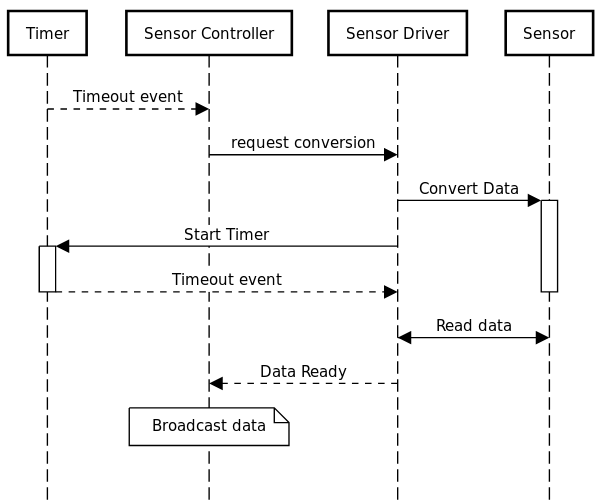
\includegraphics[width=0.65\linewidth]{sensor_op.png}
	\captionof{figure}{Sequência de operações dos sensores}
	\label{fig:sensor_op}
\end{center} 

Quando a leitura do sensor é obtida pelo driver um evento é gerado para o Sensor
Controller, que armazena este valor numa variável e gera um evento para os
outros módulos do software que utilizam estes valores.

Assim como o Sensor Controller, todos os drivers para os sensores foram
implementados seguindo o mesmo padrão de operação através de interrupções.

\subsubsubsection{Bluetooth Broadcaster}

O Advertising Controller, responsável pela operação do modo Broadcaster, possui
dependências com as bibliotecas do SDK responsáveis pela codificação dos pacotes
e chamadas de funções do SoftDevice.

Este controlador oferece interfaces, como mostra o código fonte
\ref{lst:adv_ctrl_interface}, para as configurações do intervalo de transmissão
e potência de rádio, bem como a interface que recebe os eventos de dados dos
sensores, utilizado para atualizar o pacote de dados transmitido pelo
dispositivo, além de oferecer as chamadas para a inicialização deste módulo.

\begin{minipage}{0.95\linewidth} 
\lstinputlisting[firstline=13,lastline=20,label={lst:adv_ctrl_interface},
caption={Interface do Advertising Controller}] 
{../Development/ble-sensor-station/src/libs/ble/advertising/ble_adv_controller.h}
\end{minipage}

A inicialização deste componente de software configura as informações do pacote
não relacionadas ao conteúdo. São estas configurações: intervalo padrão de
advertising, duração do período conectável do dispositivo e advertising público
e não direcionado. O SDK oferecido pela Nordic Semiconductor considera que
quando o valor de Timeout para o período conctável é 0 o dispositivo permanecerá
conectável durante todo o ciclo de operação\cite{nrf51sdkManual}. O código fonte
\ref{lst:adv_ctrl_init} mostra a inicialização deste componente com intervalo de
transmissão inicial de 200ms.

As configurações referentes ao Device Name e MAC Address são definidas pelo
bloco da arquitetura BLE Manager.

\begin{minipage}{0.95\linewidth} 
\lstinputlisting[firstline=71,lastline=82,label={lst:adv_ctrl_init},
caption={Rotina de inicialização do Advertising Controller}]
{../Development/ble-sensor-station/src/libs/ble/advertising/ble_adv_controller.c}
\end{minipage}

A função \dblquote{update\_adv\_data()} é responsável por preparar os dados do
pacote de advertising e scan response, disponibilizando-os para as bibliotecas
referentes à operação do rádio construirem o pacote bluetooth, como mostra o código fonte
\ref{lst:adv_update_data}.

\begin{minipage}{0.95\linewidth} 
\lstinputlisting[firstline=102,lastline=122,label={lst:adv_update_data},
caption={Preparação dos dados de Advertising e Scan Response}] 
{../Development/ble-sensor-station/src/libs/ble/advertising/ble_adv_controller.c}
\end{minipage}

Os pacotes são contruídos de acordo com o projetado, sendo o pacote de
advertising formado pelas flags que indicam operação somente no Bluetooth Low
Energy (LE\_ONLY) e mantendo a flag de General Discovery Mode ativa
(GENERAL\_DISC\_MODE), indicando que o dispositivo aceita conexões enquanto
estiver operando. O pacote de advertising também recebe o endereço para a
variável \dblquote{manuf\_data}, que contém o Company ID, o ponteiro para o
pacote de dados para ser enviado e o tamanho deste pacote, que está de acordo
com a tabela \ref{tab:adv_template}.

Quando o Advertising Controller recebe um evento de dados dos sensores através
da função \dblquote{adv\_on\_sensor\_evt} é executada a rotina presente no
código fonte \ref{lst:adv_ctrl_sensor_evt}, atualizando os valores da estrutura
de dados que armazena os dados para a codificação no pacote de advertising.

\begin{minipage}{0.95\linewidth} 
\lstinputlisting[firstline=48,lastline=68,label={lst:adv_ctrl_sensor_evt},
caption={Rotina de atualização dos dados dos sensores}]
{../Development/ble-sensor-station/src/libs/ble/advertising/ble_adv_controller.c}
\end{minipage}

As funções de configuração para intervalo de advertising, potência do rádio e de
início/parada de advertising se resumem a chamadas das bibliotecas do SDK.

\subsubsubsection{Bluetooth Slave}




A operação no modo Bluetooth Slave ocorre principalmente através do tratamento
de eventos ocorridos pela interação com o usuário.

\subsubsubsection{BLE Manager}
PENDING

%End of Sensor Station

\subsubsection{Gateway Bluetooth - Internet}
PENDING
% 			-> Hardware
% 			-> Ambiente de desenvolvimento
%end of BLE-Internet gateway

\subsubsection{Infraestrutura online}

A infraestrutura online foi configurada utilizando a interface online do Amazon
AWS IoT Core, que é disponibilizada após o cadastro na plataforma.

As principais tarefas de desenvolvimento nessa interface são: a criação de um
dispositivo, a criação dos certificados de segurança e a criação de políticas de
acesso.

Na figura \ref{fig:aws_creating_thing} é mostrada a interface utilizada para a
criação de um dispositivo. Ao criá-lo, é possível escolher opções como nome
e tipo de dispositivo. Ao final da criação, pede-se para associar o dispositivo
criado a um certificado de segurança. Quando nenhum certificado é encontrado na
conta do usuário, é oferecida a criação de um certificado em um clique.

\begin{center}
	\centering 
	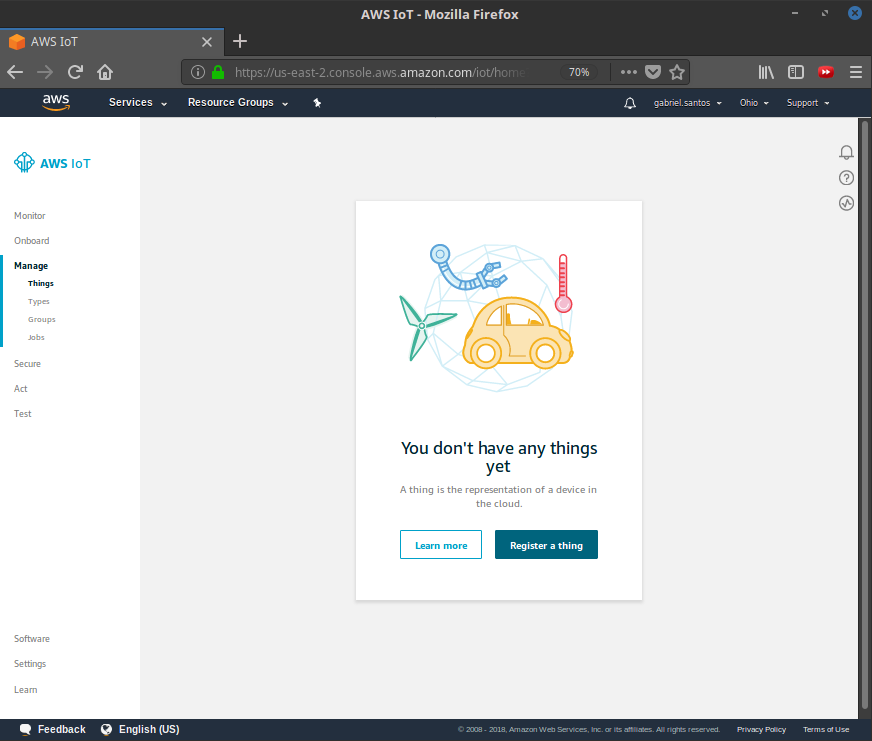
\includegraphics[width=0.85\linewidth]{creating_thing.png}
	\captionof{figure}{Interface online do AWS IoT Core para criação de
	dispositivos}
	\label{fig:aws_creating_thing}
\end{center} 

Quando um certificado é criado, abre-se uma página de download que permite a
realização do download do certificado e das chaves de segurança utilizadas na
criptografia. Quando um certificado é feito durante a criação de um dispositivo,
eles são associados autimaticamente. Caso contrário, a associação deve ser feita
manualmente. A figura \ref{fig:aws_cert_dl} mostra a página de download do
certificado.

\begin{center}
	\centering 
	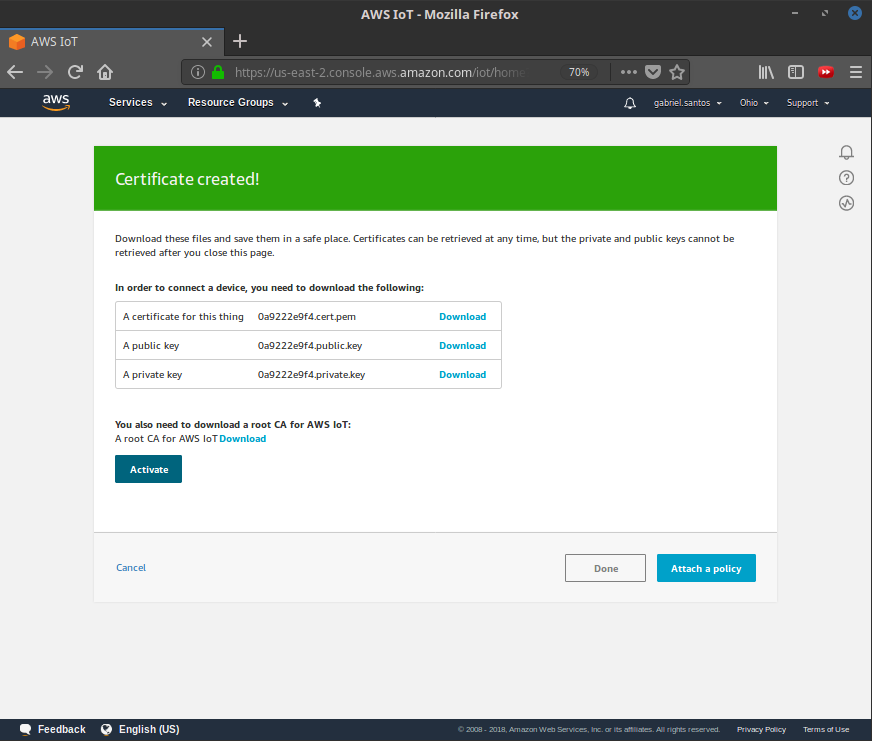
\includegraphics[width=0.85\linewidth]{cert-created.png}
	\captionof{figure}{Página de criação do certificado}
	\label{fig:aws_cert_dl}
\end{center} 



PENDING
% -> Ambiente de desenvolvimento	
% -> Coleta e armazenamento de dados
%end of infrastructure
%end of implementation


